\chapter{Conference and Local Information}

\setlength\fboxsep{0pt}
\setlength\fboxrule{0.5pt}
%\phantomsection \section{Help and Emergencies}

%In case of an emergency at the conference, please call {\Large \textbf{911}}. You can also request help from any of the conference volunteers and the concierge at the main entrances of university buildings. For emergencies at the conference or elsewhere in USA, please call the emergency number {\Large \textbf{911}}. 

%If you need special assistance to access a building, please contact the registration desk at {\Large \textbf{NUMBER}}.

\vspace{-1.0cm}
\phantomsection \section{General Information}

\section*{About Berkeley}

Berkeley (pronounced burk-lee) is a city on the east shore of San Francisco Bay in northern Alameda County, California, that is named after the eighteenth-century bishop and philosopher George Berkeley. Berkeley borders the cities of Albany, Oakland, and Emeryville and Contra Costa County including unincorporated Kensington as well as San Francisco Bay. According to the United States Census Bureau the city's 17.7 square miles area includes 10.5 square miles of land and 7.2 square miles water, most of it part of San Francisco Bay. Its population at the 2010 census was determined to be 112,580 and it is one of the most politically liberal cities in the United States.

Berkeley is the site of the oldest campus in the University of California system – the University of California, Berkeley – and of the Lawrence Berkeley National Laboratory that the university manages and operates. 

Berkeley is served by Amtrak (Capitol Corridor), AC Transit, BART (Ashby, Downtown Berkeley Station and North Berkeley) and bus shuttles operated by major employers including UC Berkeley and Lawrence Berkeley National Laboratory. The Eastshore Freeway (Interstate 80 and Interstate 580) runs along the bay shoreline. Berkeley also hosts car sharing networks run by City CarShare, Uhaul Car Share, and Zipcar. Several "pods" (points of departure where cars are kept) exist throughout the city, in several downtown locations, at the Ashby and North Berkeley BART stations, and at various other locations in Berkeley (and other cities in the region).

Berkeley has a number of distinct neighborhoods. Surrounding the University of California campus are the most densely populated parts of the city. West of the campus is Downtown Berkeley, the city's traditional commercial core; home of the civic center, the city's only public high school, the busiest BART station in Berkeley, as well as a major transfer point for AC Transit buses. South of the campus is the Southside neighborhood, mainly a student ghetto, where much of the university's student housing is located. The busiest stretch of Telegraph Avenue is in this neighborhood. North of the campus is the quieter Northside neighborhood, the location of the Graduate Theological Union. North of Downtown is the North Berkeley neighborhood, which has been nicknamed the "Gourmet Ghetto" because of the concentration of well-known restaurants and other food-related businesses. In the southeastern corner of the city is the Claremont District, home to the Claremont Hotel; and the Elmwood District, with a small shopping area on College Avenue. West of Elmwood is South Berkeley, known for its weekend flea market at the Ashby Station. The areas of South and West Berkeley are in the midst of redevelopment. Along the shoreline of San Francisco Bay at the foot of University Avenue is the Berkeley Marina. 

\vspace{3mm}
\section*{About University of California, Berkeley}

The University of California, Berkeley (also referred to as UC Berkeley; Berkeley; California; or simply Cal), is a public research university located in Berkeley, California. The university occupies 1,232 acres (499 ha) on the eastern side of the San Francisco Bay with the central campus resting on 178 acres (72 ha). Berkeley is the flagship institution of the 10 campus University of California system.

Established in 1868 as the result of the merger of the private College of California and the public Agricultural, Mining, and Mechanical Arts College in Oakland, Berkeley is the oldest institution in the UC system and offers approximately 350 undergraduate and graduate degree programs in a wide range of disciplines. Berkeley has been charged with providing both "classical" and "practical" education for the state's people. Berkeley co-manages three United States Department of Energy National Laboratories, including the Los Alamos National Laboratory, Lawrence Livermore National Laboratory and Lawrence Berkeley National Laboratory for the U.S. Department of Energy.

%Berkeley faculty, alumni, and researchers have won 72 Nobel Prizes (including 30 alumni Nobel laureates), 9 Wolf Prizes, 7 Fields Medals, 15 Turing Awards, 45 MacArthur Fellowships, 20 Academy Awards, and 11 Pulitzer Prizes. 

\vspace{3mm}

\section*{Registration}

The registration desk will be located in the lobby of Wheeler Hall on the first floor. Student volunteers will be present at the desk and will provide you with a registration packet consisting of your name tag, wireless internet access credentials, a printed conference booklet, conference t-shirt, and tickets to the conference banquet and the Dinner \& Demos event at Google HQ.

\vspace{3mm}
\section*{Wireless Internet Access}
Conference participants will be able to access the campus-wide wireless \emph{AirBears} network. Access credentials are printed on your name tag. If you have difficulties setting up your wireless access, please contact any of the volunteers or the registration desk.

\vspace{3mm}
\section*{Help and Emergencies}
In case of an emergency at the conference, you can seek assistance from any of the conference volunteers (who will wear gold t-shirts) or seek assistance at the registration desk. For medical emergencies at the conference, please call 911.

\clearpage
\phantomsection \section{Conference and Workshops Venues}
%The following campus map shows the location.
\begin{figure}[h!]
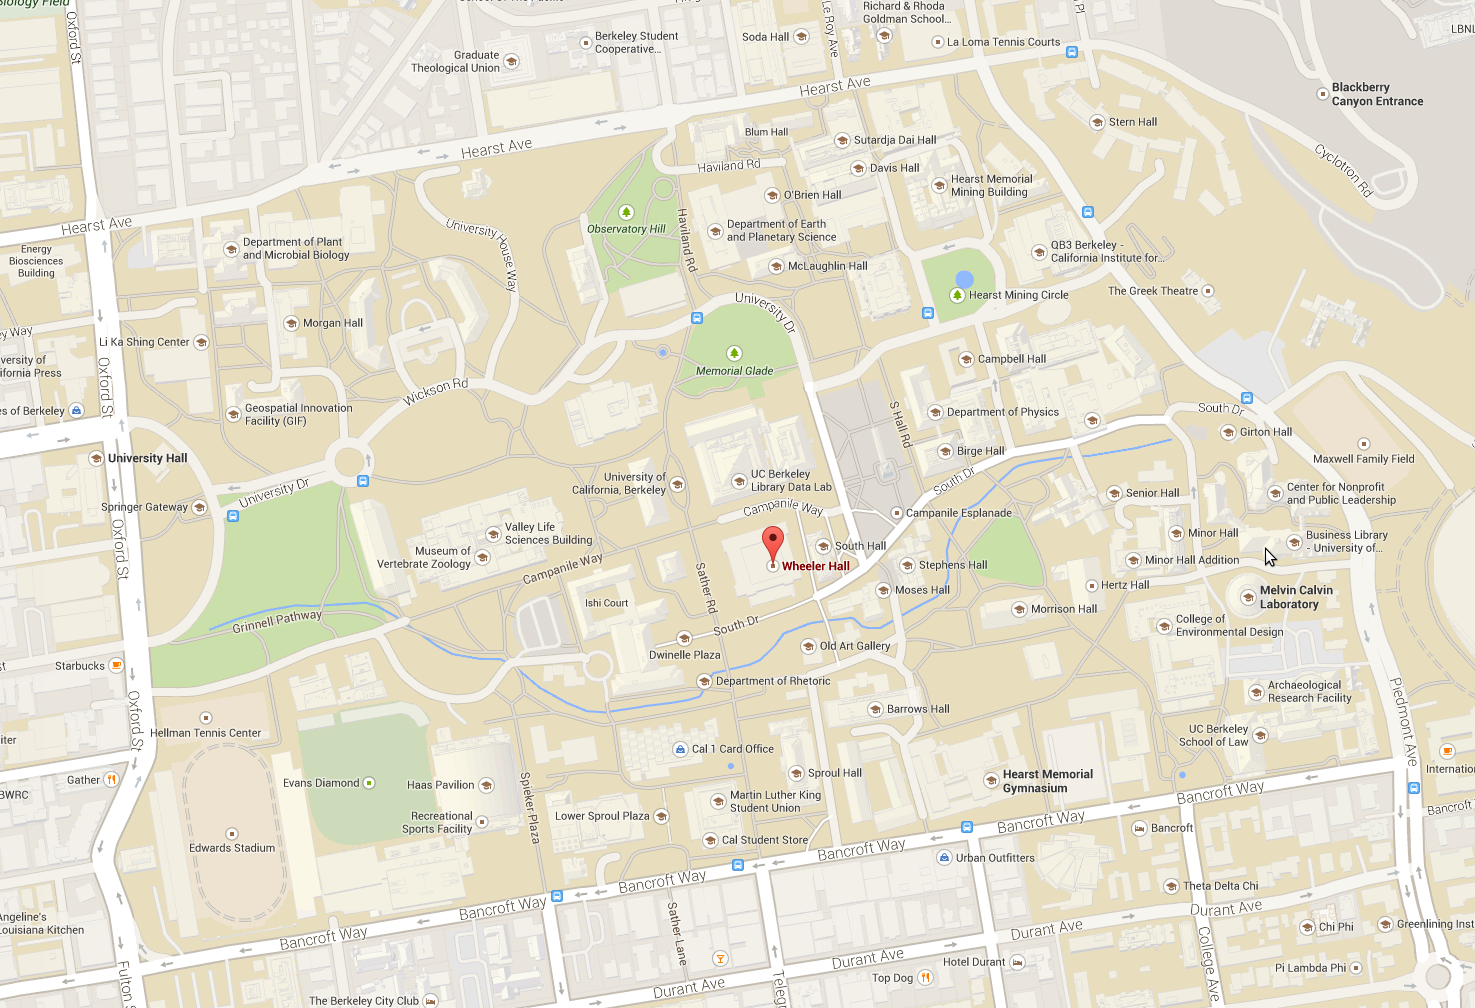
\includegraphics[width=\linewidth]{local_img/maps/wheeler_hall}
\end{figure}
\vspace{0.3cm}
{\Large The conference and workshops will take place in Wheeler Hall on the UC Berkeley campus.}

\newpage
\phantomsection \section{1st Floor -- Conference and Workshops Venue}
{\large Monday, July 14 to Wednesday, July 16}
\begin{figure}[h!]
\center
\includegraphics[height=0.6\textheight]{local_img/maps/first_floor}
\end{figure}

\vspace{0.3cm}

{\Large \textbf{Legend}: 
\begin{itemize}
\itemsep0em 
\item Gold: Rooms in use 
\item Blue: Restrooms
\item Gray: Rooms not in use
\end{itemize}
}

\vspace{0.3cm}
{\Large The registration desk will be located in the lobby of Wheeler Hall.}

\vspace{0.3cm}
{\Large Please see Technical Program for conference and workshop room assignments.}

\newpage
\phantomsection \section{Basement Floor -- Workshops Venue}
{\large Saturday, July 12 to Sunday, July 13}

\begin{figure}[h!]
\center
\includegraphics[height=0.6\textheight]{local_img/maps/basement}
\end{figure}

\vspace{0.3cm}

{\Large \textbf{Legend}: 
\begin{itemize}
\itemsep0em 
\item Gold: Rooms in use 
\item Blue: Restrooms
\item Gray: Rooms not in use
\end{itemize}
}

\vspace{0.3cm}
{\Large Please see Technical Program for workshop room assignments.}

\newpage
\phantomsection \section{2nd Floor -- Workshops Venue}
{\large Saturday, July 12 to Sunday, July 13}

\begin{figure}[h!]
\center
\includegraphics[height=0.6\textheight]{local_img/maps/second_floor}
\end{figure}

\vspace{0.3cm}

{\Large \textbf{Legend}: 
\begin{itemize}
\itemsep0em 
\item Gold: Rooms in use 
\item Blue: Restrooms
\item Gray: Rooms not in use
\end{itemize}
}

\vspace{0.3cm}
{\Large Please see Technical Program for workshop room assignments.}


\newpage
\phantomsection \section{Special Events}

\section*{Welcome Reception (Sponsored by Anki)}

We will celebrate the 10th edition of RSS with cake and drinks. Anki will have demos of the Anki Drive game for RSS attendees to try out.

\vspace{3mm}
\section*{Conference Banquet}
The conference banquet will be held on a cruise on the San Francisco Bay. Enjoy a splendid sunset on the water with magnificent views of the city of San Francisco, accompanied by a delicious seasonal dinner and drinks. Transportation will be provided. Buses will pick us up from Berkeley at 6pm and take us to Pier 3 in San Francisco, where we will board the San Francisco Belle. Buses will pick us up from Pier 3 around 10pm, and we'll be back in Berkeley around 10:30pm.

\vspace{3mm}
\section*{Dinner \& Demos at Google HQ}
On the last day of the conference, Google will be hosting a special evening event for RSS attendees at the Google Headquarters in Mountain View. You can look forward to a night of hosted dinner and demos from some of the Google teams working on robotics, machine learning, and computer vision. Teams that will be present include the Self-Driving Car team, Project Loon, Google Glass, Streetview, and more. Transportation will be provided. Buses will pick us up from Berkeley at 5pm and take us to Mountain View. Storage for luggage will be provided at the venue. Buses will bring us back to Berkeley around 10pm.


%set back fbox frame
\setlength\fboxrule{0pt}


\begin{figure}[h!]
\center
\fbox{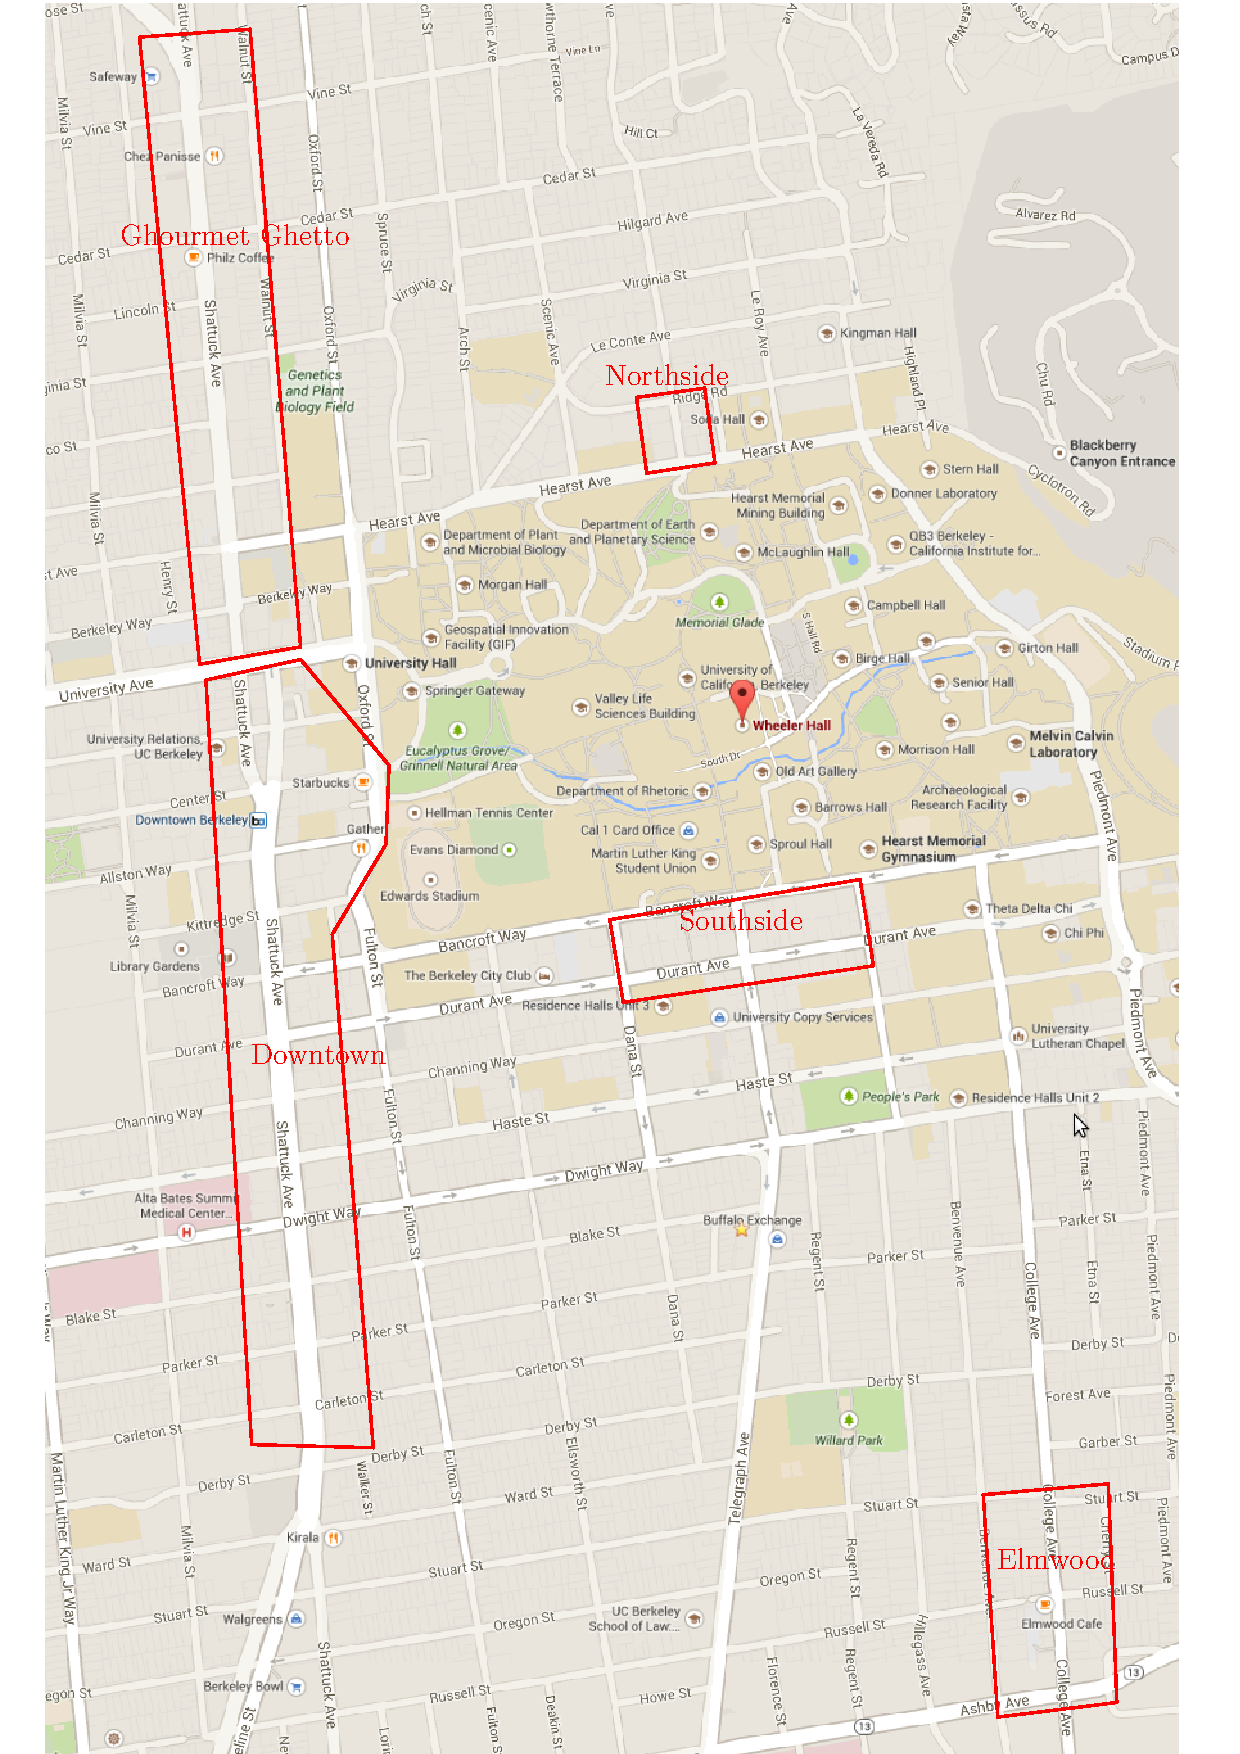
\includegraphics[width=6in]{local_img/maps/food.pdf}}
\end{figure}
